\documentclass[fontsize=12pt, paper=a4, headinclude, twoside=false, parskip=half+, pagesize=auto, numbers=noenddot, open=right, toc=listof, toc=bibliography]{scrreprt}
% PDF-Kompression
\pdfminorversion=5
\pdfobjcompresslevel=1
% Allgemeines
\usepackage[automark]{scrpage2} % Kopf- und Fußzeilen
\usepackage{amsmath,marvosym} % Mathesachen
\usepackage[T1]{fontenc} % Ligaturen, richtige Umlaute im PDF
\usepackage[utf8]{inputenc}% UTF8-Kodierung für Umlaute usw
% Schriften
\usepackage{mathpazo} % Palatino für Mathemodus
\usepackage{setspace} % Zeilenabstand
\onehalfspacing % 1,5 Zeilen
% Schriften-Größen
\setkomafont{chapter}{\Huge\rmfamily} % Überschrift der Ebene
\setkomafont{section}{\Large\rmfamily}
\setkomafont{subsection}{\large\rmfamily}
\setkomafont{subsubsection}{\large\rmfamily}
\setkomafont{chapterentry}{\large\rmfamily} % Überschrift der Ebene in Inhaltsverzeichnis
\setkomafont{descriptionlabel}{\bfseries\rmfamily} % für description Umgebungen
\setkomafont{captionlabel}{\small\bfseries}
\setkomafont{caption}{\small}
% Sprache: Deutsch
\usepackage[ngerman]{babel} % Silbentrennung
\usepackage{csquotes} % quotes
% PDF
\usepackage[ngerman]{hyperref}
\addto\extrasngerman{% Umbenennung der Kapitel Referenzen
  \def\subsectionautorefname{Abschnitt}%
  \def\subsubsectionautorefname{Abschnitt}%
}
\usepackage[final]{microtype} % mikrotypographische Optimierungen
\clubpenalty = 10000 
\widowpenalty = 10000 
\displaywidowpenalty = 10000
\usepackage{url}
\renewcommand*{\UrlFont}{\footnotesize}
\usepackage{pdflscape} % einzelne Seiten drehen können
% Tabellen
\usepackage{multirow} % Tabellen-Zellen über mehrere Zeilen
\usepackage{multicol} % mehre Spalten auf eine Seite
\usepackage{tabularx} % Für Tabellen mit vorgegeben Größen
\usepackage{longtable} % Tabellen über mehrere Seiten
\usepackage{array}
\usepackage{float}
%  Bibliographie
\usepackage{bibgerm} % Umlaute in BibTeX
\usepackage{natbib}
% Bilder
\usepackage{graphicx} % Bilder
\usepackage{color} % Farben
\usepackage{xcolor,colortbl} % Text Hintergrundfarben und Tabellenfarben
\usepackage{varwidth}
\usepackage{changepage}
\graphicspath{{images/}}
\DeclareGraphicsExtensions{.pdf,.png,.jpg} % bevorzuge pdf-Dateien
\usepackage{subcaption}  % mehrere Abbildungen nebeneinander/übereinander
\usepackage[all]{hypcap} % Beim Klicken auf Links zum Bild und nicht zu Caption gehen
% Bildunterschrift
\setcapindent{0em} % kein Einrücken der Caption von Figures und Tabellen
\setcapwidth{0.9\textwidth} % Breite der Caption nur 90% der Textbreite, damit sie sich vom restlichen Text abhebt
\setlength{\abovecaptionskip}{0.2cm} % Abstand der zwischen Bild- und Bildunterschrift
% Quellcode
\usepackage{listings} % für Formatierung in Quelltexten
\usepackage{DejaVuSansMono} % ttfamily font
\usepackage{todonotes}% Todo Notes
\presetkeys{todonotes}{inline}{}
% Bibliography multicoloumn
\usepackage{etoolbox}
\usepackage{relsize}
\patchcmd{\thebibliography}{\list}{\begin{multicols}{2}\small\list}{}{}\appto{\endthebibliography}{\end{multicols}}

\definecolor{gray}{rgb}{0.5,0.5,0.5}
\definecolor{orange}{rgb}{.99,0.5,0}
\definecolor{green}{rgb}{0,0.4,0}
\definecolor{lightgreen}{rgb}{0.7,1,0.7}
\definecolor{codegreen}{rgb}{0,0.6,0}
\definecolor{codegray}{rgb}{0.5,0.5,0.5}
\definecolor{backcolour}{rgb}{0.97,0.97,0.95}

\lstdefinestyle{mystyle}{
  inputencoding={utf8},
  xleftmargin=1em,
  backgroundcolor=\color{backcolour},   
  basicstyle=\tiny\ttfamily,
  commentstyle=\color{gray},
  keywordstyle=\color{green}\textbf,
  numberstyle=\tiny\color{codegray},
  stringstyle=\color{orange},
  breakautoindent  = true,
  breakindent      = 2em,
  breaklines       = true,
  postbreak        = ,
  prebreak         = \raisebox{-.8ex}[0ex][0ex]{\Righttorque},                
  captionpos=b,                    
  keepspaces=true,                 
  numbers=left,                    
  numbersep=5pt,
  numberstyle=\tiny\ttfamily\color{gray},               
  showspaces=false,                
  showstringspaces=false,
  showtabs=false,                  
  tabsize=2,
  literate=%
    {Ö}{{\"O}}1
    {Ä}{{\"A}}1
    {Ü}{{\"U}}1
    {ß}{{\ss}}1
    {ü}{{\"u}}1
    {ä}{{\"a}}1
    {ö}{{\"o}}1
    {~}{{\textasciitilde}}1
}
\lstset{style=mystyle}
% linksbündige Fußboten
\deffootnote{1.5em}{1em}{\makebox[1.5em][l]{\thefootnotemark}}

\typearea{14} % typearea berechnet einen sinnvollen Satzspiegel (das heißt die Seitenränder) siehe auch http://www.ctan.org/pkg/typearea. Diese Berechnung befindet sich am Schluss, damit die Einstellungen oben berücksichtigt werden
\textwidth=440pt % text width

\usepackage{scrhack} % Vermeidung einer Warnung
\usepackage{acronym} % Abkürzungsverzeichnis

% chapter margin
\renewcommand*{\chapterheadstartvskip}{\vspace*{0cm}}
\renewcommand*{\chapterheadendvskip}{\vspace{.5cm}}


% Eigene Befehle %%%%%%%%%%%%%%%%%%%%%%%%%%%%%%%%%%%%%%%%%%%%%%%%%5
% Matrix
\renewcommand*{\i}[1]{%
      {\textit{#1}}%
}
\renewcommand*{\b}[1]{%
      {\textbf{#1}}%
}
\renewcommand*{\tt}[1]{%
      {\footnotesize\texttt{#1}}%
}
\newcommand{\q}[1]{%
      {\enquote{#1}}%
}
\newcommand{\sq}[1]{%
      {\enquote*{#1}}%
}

% break inside a table cell
\newcommand{\br}[3]{%
      {\parbox{#1cm}{#2\\#3\vspace{3pt}}}%
}

\newcommand{\mat}[1]{%
      {\textbf{#1}}%
}
\newcommand{\info}[1]{
      {\colorbox{blue}{ (INFO: #1)}}
}
% Hinweis auf Programme in Datei
\newcommand{\datei}[1]{%
      {\ttfamily{#1}}%
}
\newcommand{\code}[1]{%
      {\footnotesize\ttfamily{\colorbox{gray!20}{\begin{varwidth}{\dimexpr\linewidth-2\fboxsep}#1\end{varwidth}}}}%
}
% bild mit defnierter Breite einfügen
\newcommand{\bild}[4]{
  \begin{figure}[H]
    \centering
      \vspace{1ex}
      \includegraphics[width=#2]{images/#1}
      \caption[#4]{\label{img.#1} #3}
    \vspace{1ex}
  \end{figure}
}
% bild mit defnierter Breite und Leftshift einfügen
\newcommand{\bildl}[5]{
  \begin{figure}[H]
    \centering
      \vspace{1ex}
      \hspace*{#3}
      \includegraphics[width=#2]{images/#1}
      \caption[#5]{\label{img.#1} #4}
    \vspace{1ex}
  \end{figure}
}
% bild mit eigener Breite
\newcommand{\bilda}[3]{
  \begin{figure}[H]
    \centering
      \vspace{1ex}
      \includegraphics{images/#1}
      \caption[#3]{\label{img.#1} #2}
      \vspace{1ex}
  \end{figure}
}
 % import preamble config
% start document
\begin{document}
\pagenumbering{arabic} % große Römische Seitenummerierung
\pagestyle{empty}

% title page
\clearscrheadings\clearscrplain
\begin{center}

\includegraphics[width=0.28\textwidth]{images/logo_tu_berlin}
\vspace{8mm}

{\huge Technische Universität Berlin}\\
\vspace{2mm}
{\large Quality and Usability Lab}\\
% \vspace{1mm}
% {\large Institute of Software Engineering\\and Theoretical Computer Science}\\
\vspace{11mm}

{\Huge Part-of-Speech Tagging\\[-2mm] with Neural Networks\\[-2mm] for a Conversational Agent\\}
\vspace{20mm}
{\Huge \b{Master Thesis}}\\
{\b{Master of Science (M.Sc.)}}\\
\vspace{24mm}
\begin{tabular}{rl}
  \b{Author} & Andreas Müller\\
  \b{Major} & Computer Engineering\\
  \b{Matriculation No.} & 333471\\
   & \\
  \b{Date} & 18th May 2018 \\
  \b{1st supervisor} & Prof. Dr.-Ing. Sebastian Möller \\
  \b{2nd supervisor} & Dr. Axel Küpper \\
\end{tabular}

\end{center}
\clearpage
\pagestyle{scrheadings} % normale Kopf- und Fußzeilen für den Rest

% ===================================================================================
\BlankPage

% ===================================================================================
\chapter*{Eidesstattliche Erklärung}
Hiermit versichere ich, dass ich die vorliegende Arbeit selbstständig verfasst und keine anderen als die angegebenen Quellen und Hilfsmittel benutzt habe. Alle Ausführungen, die anderen veröffentlichten oder nicht veröffentlichten Schriften wörtlich oder sinngemäß entnommen wurden, habe ich kenntlich gemacht.

Die Arbeit hat in gleicher oder ähnlicher Fassung noch keiner anderen Prüfungsbehörde vorgelegen.
\vspace{10mm}

Berlin, den \today\\

\vspace{1cm}
\rule{.5\textwidth}{.5pt}\\
Unterschrift

% ===================================================================================
\BlankPage

% ===================================================================================
\chapter*{Abstract}
A part-of-speech tagger is a system which automatically assigns the part of speech to words using contextual information. Potential applications for part-of-speech taggers exist in many areas of computational linguistics including speech recognition, speech synthesis, machine translation or information retrieval in general.

The part-of-speech tagging task of natural language processing is also used in the advisory artificial conversational agent called \Alex. \Alex\ was developed to answer questions about modules and courses at the Technische Universität Berlin. The system takes the written natural language requests from the user and tries to transform them into SQL-queries. To understand the natural language queries, the system uses a Hidden Markov Model (HMM) to assign tags to each word of the query (part-of-speech tagging). This HMM tagger is trained with manually created training templates that are filled with the data in the database to be queried. The manually created sentence-templates and the slot-filling resulted in many training data sentences with the same structure. This often led to wrong tagging results when the HMM tagger was presented with an input sentence, having a structure that doesn't occur in the training templates.

This thesis shows two different neural network approaches for the language modeling of the input sentences and evaluates and compares both neural network based tagger as well as the HMM based tagger.

% ===================================================================================
\BlankPage

% ===================================================================================
\chapter*{Zusammenfassung}
Ein Part-of-speech Tagger ist ein System, welches Wortarten anhand von Kontextinformationen automatisch den gegebenen Wörtern zuordnet. Potentielle Anwendungen solcher Tagger gibt es in vielen Bereichen der Computerlinguistik wie Spracherkennung, Sprachsynthese, maschinelle Übersetzung oder Information Retrieval im Allgemeinen.

Part-of-speech Tagging wird auch in \Alex\ verwendet, einem Artificial Conversational Agent. \Alex\ wurde entwickelt, um Fragen zu Modulen und Lehrveranstaltungen an der Technischen Universität Berlin zu beantworten. Das System nimmt die in natürlicher Sprache geschriebenen Anfragen des Benutzers und versucht diese in SQL-Abfragen umzuwandeln. Um die natürliche Sprache zu verstehen, verwendet das System ein Hidden-Markov-Model (HMM), um jedem Wort der Eingabe Wortarten zuzuweisen (Part-of-speech Tagging). Dieser HMM-Tagger wird mit manuell erstellten Trainingsvorlagen trainiert, die mit den Daten der abzufragenden Datenbank gefüllt werden. Die manuell erstellten Satzvorlagen führten zu vielen Trainingsdatensätzen mit gleicher Struktur und damit oft zu falschen Tagging-Ergebnissen, wenn der HMM-Tagger einen Eingabesatz mit einer Struktur verarbeiten sollte, die in den Trainingsvorlagen nicht vorkommt.

Diese Arbeit zeigt zwei verschiedene Ansätze für die Sprachmodellierung der Eingabesätze basierend auf neuronalen Netzwerken und bewertet und vergleicht sowohl die Neuronalen Netzwerk-basierten Tagger als auch den HMM-basierten Tagger.

% ===================================================================================
\BlankPage

% ===================================================================================
\tableofcontents

% ===================================================================================
\listoffigures

% ===================================================================================
\listoftables

% ===================================================================================
\chapter*{Abbreviations}\label{s.abbr}
\addcontentsline{toc}{chapter}{Abbreviations}
\markboth{Abbreviations}{Abbreviations}
\begin{acronym}[----------------]
 \acro{ACA}{\i{Artificial Conversational Agent}}
 \acro{ANN}{\i{Artificial Neural Network}}
 \acro{FNN}{\i{Feed-forward Neural Network}}
 \acro{HMM}{\i{Hidden Markov Model}}
 \acro{NLP}{\i{Natural Language Processing}}
 \acro{NLTK}{\i{Natural Language Toolkit}}
 \acro{RNN}{\i{Recurrent Neural Network}}
\end{acronym}

% ===================================================================================
\chapter{Introduction}\label{c.introduction}
% Turing: Artificial Intelligence
% Brown: NLP
% POS Tagging

\i{Learning} is one of the most essential parts of human life. From the beginning to the end human beings acquire knowledge and skills. Learning means progress, additional value, failing and repeating. It enables growth and improvement.

In biology, learning is based on a specific strengthening of the connection of certain nerve cells in the central nervous system by facilitating signal transmission at the synapses through appropriate modifications. Being a huge amendable network of connected neurons the nervous system served as a role model for a research field called \i{Machine Learning}. This term was coined by A. Samuel\footnote{Arthur Lee Samuel was an early researcher in machine learning and artificial intelligence. He developed the first successful self-learning program: the Samuel-Checkers game \cite{samuel1959}.} \cite{samuel1959} in 1959, who distinguished two general approaches to the problem of machine learning: a general-purpose randomly connected Neural Network approach and a special-purpose highly organized network. Following a publication of  W. McCulloch about the comparison of a computer with the nervous system of a flatworm in 1949 \cite{mcculloch1949}, he stated:

\i{``A comparison between the size of the switching nets\\that can be reasonably constructed or simulated at the present time\\and the size of the neural nets used by animals,\\suggests that we have a long way to go before we obtain practical devices.''}\\
\parbox{\textwidth}{\hfill \hfill -- Arthur Lee Samuel (1959)}

Less than 60 years later, today we have a lot of practical devices using machine learning and artificial intelligence technologies in our everyday life. Especially the processing and understanding of spoken or written natural language has a wide range of applications. One of those applications are advisory artificial conversational agents (ACA), chat-bots in short. They are designed to give natural language answers to natural language questions, making it as easy as possible for users to interact with a special system. \Alex\ is an example of an ACA that is able answer questions about courses and modules of the TU Berlin. This thesis aims to improve the understanding and learning of natural language of \Alex\ with artificial neural networks.

\section{Scope of this Thesis}\label{c.introduction.scope}
The scope of this thesis is the development of a neural network based part-of-speech tagger for the advisory Artificial Conversational Agent \Alex, the training of different language models and their evaluation with corresponding test sets.

In order to accomplish the new language models, two different neural network architectures are implemented: A feed-forward neural network and a recurrent neural network. For the training of both neural network implementations, a corpus of tagged language data is generated with the help various input templates, which are created on the basis of logged user input data.

To evaluate the language models, a data set of known data\footnote{Data, that was already used for the training of the model} and unknown data\footnote{Data, that includes words and sentence structures, that didn't occur in the training data sets} is created. On the basis of this evaluation, both neural network models and the HMM are compared to each other.

In accordance to the evaluation results, the former HMM based part-of-speech tagger is then replaced by this new tagger. To guarantee a seamless integration, the new tagger is implemented as a separate module with the same program interface the old tagger already utilizes. This way no other components of the conversational agent have to be changed and the effort of the replacement is kept minimal.

\section{Related Work}\label{c.introduction.related}
This thesis is build upon the work of T. Michael \cite{michael2016}, who describes the design and implementation of \Alex\ in detail. The conversational agent was implemented for the purpose of helping students of the TU Berlin to organize their studies by providing a simple way to gain information about modules and courses. It utilizes two separate already existing baseline systems by merging their data into one relational database. This database is  used as the central access point for the information that users want to retrieve.

\begin{figure}[H]
	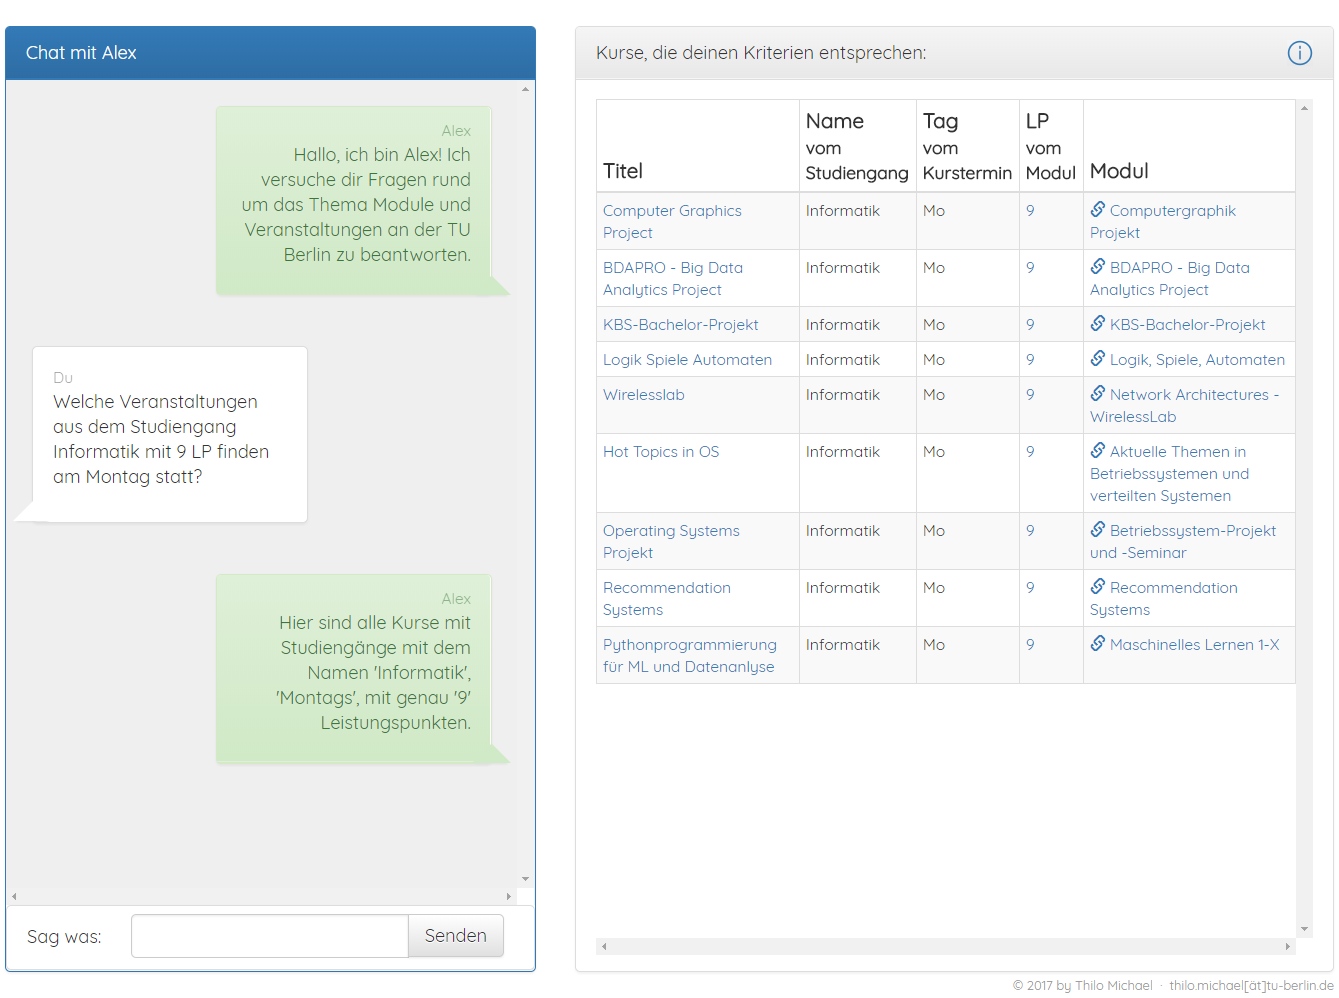
\includegraphics[width=\textwidth]{images/alex_screencapture}
	\caption[User Interface of \Alex]{The user interface of \Alex. The left section contains the conversation with the Agent and a field where the user can type. The right section shows the result of the generated database query in tabular form.\\The user asked for all courses of the subject \i{computer science} that provide 9 ECTS and are scheduled on a Monday. The agent answered accordingly.\\This image was captured at the 21st April 2018.}
	\label{f.alex_ui}
\end{figure}

\Alex\ consists of several processing modules:

\begin{itemize}
	\item The \b{tagging module} uses a Hidden Markov Model to calculate the parts of speech for the user input, later described in chapter \ref{c.alex.hmm}
	\item The \b{query generation module} composes actual SQL queries from the tagging output data by recognizing the requested model and the return type
	\item The \b{filter extraction module} provides refinement and constraint handling for the query generator
	\item The \b{response generation module} formulates answers for the user input in natural language by processing the generated query, the recognized model and the conversation state.
\end{itemize}

Moreover \Alex\ provides a user interface which utilizes web technologies and can be accessed in a web browser. Figure \ref{f.alex_ui} shows the user interface where the user asked one question and the agent returned the result in tabular form and answered accordingly.

The focus of this thesis lies on the tagging module, as the main objective is to replace the Hidden Markov Model by Artificial Neural Networks.

\subsection{The Hidden Markov Model}\label{c.introduction.related.hmm}
The Hidden Markov Model (HMM) is a probabilistic finite state machine that solves classification problems in general. It uses the observable output data of a system to derive hidden information from it. Among other applications, HMMs are used especially for speech recognition tasks.

The preliminary work for HMMs was done by R. L. Stratonovich. He first described the conditional Markov processes in 1960 \cite{stratonovich1960} that were used in the following years to describe simple Markov Models and later Hidden Markov Models (see Baum et. al. \cite{baum1966}\cite{baum1967}). The latter became popular for solving the task of automatic recognition of continuous speech \cite{baker1975} along with other applications like pattern recognition in general, the analysis of biological sequences (e.g. DNA) \cite{bishop1986} and part-of-speech tagging \cite{kupiec1992}.

\subsection{The Artificial Neural Network Model}\label{c.introduction.related.nn}
Artificial Neural Networks are networks that process information inspired by biological nervous system. They consist of connected computational units typically arranged in different layers. Such a unit (also called \i{artificial neuron}) can make calculations based on its inputs and pass the result to the next connected units. These connections are weighted, so that the weight can be adjusted depending on the activity of the unit. Thus a model of the features of the input data can be created.

After preceding research by W. McCulloch, W. Pitts \cite{mcculloch1943} and D. Hebb \cite{shaw1986} about arithmetical learning methods inspired by the connections of neurons in the 1940s, M. Minsky built the first neural network learning machine called SNARC (\i{Stochastic Neural Analog Reinforcement Computer)}\cite{crevier1993} in 1951.

In the late 1950s, F. Rosenblatt developed the \i{Mark I Perceptron} computer and published a theorem of convergence of the perceptron\cite{rosenblatt1958} in 1958. He coined the term \i{perceptron} for an algorithm that was able to learn the assignment of input data to different classes. The perceptron represents a simple artificial neural network containing one single neuron at first\footnote{Chapters \ref{c.postagging.fnn} and \ref{c.postagging.rnn} explain the architecture of different neural network structures in detail}. F. Rosenblatt stated, that every function that is representable by the model can be learned with the proposed learning method. In 1960, B. Widrow presented the ADALINE\footnote{ADALINE is an acronym for Adaptive Linear Neuron} model of a neural network, where the input weights could already be adjusted by the learning algorithm \cite{widrow1960}.

A publication of M. Minsky and S. Papert \cite{minsky1969} in 1969 analyzed and exposed some significant limitations of the basic perceptron. They pointed out, that it is not possible to learn functions without linear separability (e.g. the exclusive-or problem). Due to these limitations and the fact, that the processing power of computers at that time was not sufficient for larger neural networks, the research interest in artificial neural networks decreased in the following years.

In 1982, J. Hopfield presented a previously described Neural Network with feedback (known as \i{Hopfield network}), that was able to solve optimization problems like the \i{Traveling Salesman Problem}\footnote{The problem of the traveling salesman or round trip problem: The order of places to be visited once should be chosen in such a way that the distance covered is minimal, whereby the last place is again the starting point (round trip).}. Neural Network approaches got more attention again, also because the first processors based on transistor technology (microprocessors) came onto the market in the early 1970s and replaced the previously used tube technology in the following years, which made computers smaller and cheaper and increased their processing capacity.

For the task of POS tagging, Neural Network models were now able to outperform HMM based tagger. H. Schmid created and trained a multilayer Feed-forward Neural Network in 1994 an showed, that it performed better than an HMM tagger \cite{schmid1994}.

\section{Structure of this Thesis}\label{c.introduction.structure}
As introduction, this first chapter gave a short overview about the subject of natural language processing and part-of-speech tagging in general.

The second chapter describes structure and functionality of the already existing ACA \Alex\ with the main focus on its language model and tagging interface.

Chapter \ref{c.postagging} explains the implementation of a part-of-speech tagging system with two different neural network approaches.

The training of the language models including the retrieval of the training data and tuning of the training parameter is described in Chapter \ref{c.training}.

Chapter \ref{c.evaluation} shows the evaluation of each language model with a generated test set and their comparison.

In conclusion the final Chapter \ref{c.conclusion} discusses and summarizes the evaluation results and gives an outlook on future work.

% ===================================================================================
\chapter{\Alex: Artificial Conversational Agent}\label{c.alex}
\i{Design and Implementation of an Advisory Artificial Conversational Agent} by T. Michael \cite{michael2016} provides a detailed and comprehensive description of \Alex\ as a compilation of different modules. This chapter focuses on the modules that are relevant for the language processing and therefore adapted during this thesis.

\section{System Overview}\label{c.alex.overview}
The modular structure of \Alex\ allows the separation of different functions and therefore easier replaceability of certain functionalities. Besides a web crawler for current data retrieval for the database and a frontend interface module, \Alex\ offers a tagging module. This module provides the training of a language model as well as the assignment of tags to the words of a given input sentence.

Figure \ref{f.alex_components} shows the original architecture of \Alex.

\begin{figure}[H]
	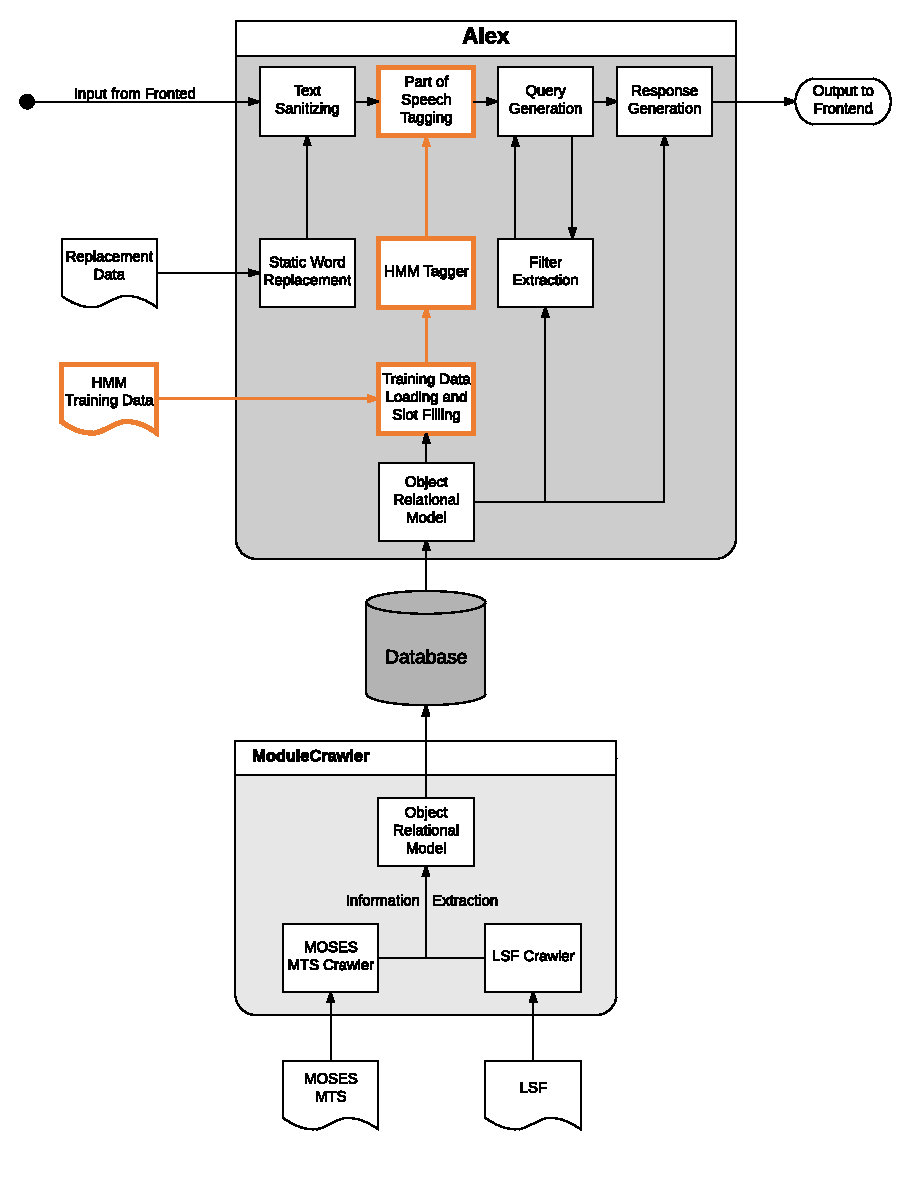
\includegraphics[width=\textwidth]{images/alex_components}
	\caption[Component Overview of \Alex]{Overview of all components of \Alex. The red colored parts are components that lie within the scope of this thesis and are adapted or replaced. Original figure by T. Michael \cite{michael2016}}
	\label{f.alex_components}
\end{figure}

\section{Training Data}\label{c.alex.data}
...

\section{The Hidden Markov Model Tagger}\label{c.alex.hmm}
As described in section \ref{c.introduction.related.hmm} \ of the introduction, the Hidden Markov Model (HMM) is a statistical tool that uses observable output data of a system to derive hidden information from it. Applications are image processing, gesture recognition and natural language processing tasks like speech recognition and part-of-speech tagging in particular.

In case of POS tagging, the observable states of the HMM represent the given sequence of words whereas the hidden states represent the corresponding parts of speech. The HMM calculates the joint probability of the whole sequence of hidden states with the help of transmission and output probabilities. Subsequently it finds the maximum probability of all possible state sequences and decides as a result, which parts of speech are most likely applied to the words of the input sequence.

Figure \ref{f.hmm_structure} illustrates an example of a state sequence with three hidden states (part of speech tags) and the observed word sequence in an HMM. The calculation of the joint probability $P$ of the word sequence in this case is shown in equation \ref{e.hmm_joint_probability} as the product of transmission and output probabilities.

\begin{equation}
    P = p_{start}\cdot p_{out,1}\cdot p_{trans,1}\cdot p_{out,2}\cdot p_{trans,2}\cdot p_{out,3} \label{e.hmm_joint_probability}
\end{equation}


\begin{figure}[H]
	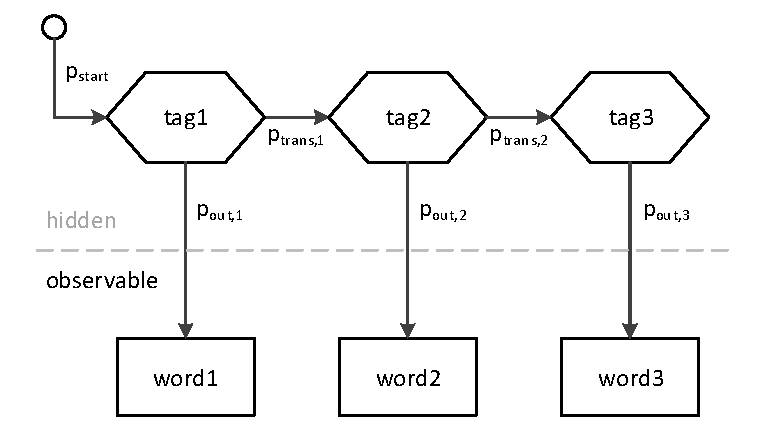
\includegraphics[width=\textwidth]{images/hmm_structure}
	\caption[Structure of a Hidden Markov Model]{An example of a state sequence of three hidden states (tag1 -- tag3) and an observed sequence of three words (word1 -- word3) in an Hidden Markov Model. $p_{start}$ denotes the start probability, $p_{trans}$ the transmission probabilities between hidden states and $p_{out}$ the output probabilities between a hidden state and an output.}
	\label{f.hmm_structure}
\end{figure}

For this purpose, an HMM is included in \Alex. According to T. Michael \cite{michael2016}, a tagging scheme was developed to extract exactly the information from a user input that is needed to successfully create a database query and return the information the user asked for. This tagging scheme was intentionally built domain independent, giving the opportunity to make \Alex\ an ACA for any topic providing a corresponding database and training data.

To maintain this universal applicability as well as the compatibility to other modules of \Alex, the Neural Network approaches presented in this thesis use the same tagging scheme \Alex\ already utilizes. For a better understanding of the evaluation results in Chapter \ref{c.evaluation}, table \ref{t.tagging_scheme} gives an overview of the 6 different classes of tags that are used by \Alex.

\begin{table}[H]
	\vspace{1ex}\small\centering\def\arraystretch{1.1}\begin{tabular}{|c|>{\raggedright}p{50mm}|p{35mm}|p{40mm}|}
	\hline
	Class & Formats & Description & Example \\
	\hline\hline
	\tt{R} & \i{Return-tags}, describing data that is expected to be returned & \tt{R\_LIST} \newline \tt{R\_SINGLE} \newline \tt{R\_COUNT} & \i{"\b{Which} modules \dots"} \newline \i{"\b{Which} module \dots"} \newline \i{"\b{How many} modules \dots"} \\ \hline
	\tt{M} & \i{Model-tags}, describing the database model, e.g. \tt{M\_MTSModule} or \tt{M\_Course} & \tt{M\_[MODEL]} & \i{"Which \b{modules} \dots"} \newline \i{"Which \b{courses} \dots"} \\ \hline
	\tt{C} & \i{Constraint-tags}, filtering the result set, given a database model and corresponding field, e.g. \tt{C\_MTSModule:ects} & \tt{C\_[MODEL]:[FIELD]} & \i{"Modules with \b{6} ects \dots"} \\ \hline
	\tt{P} & \i{Property-tags}, indicating to include fields in the result set, e.g. \tt{P\_MTSModule:ects} & \tt{P\_[MODEL]:[FIELD]} & \i{"Modules with 6 \b{ects} \dots"} \\ \hline
	\tt{Q} & \i{Comparison-tags}, describing an equal, greater than or less than constraint & \tt{Q\_EQ} \newline \tt{Q\_LT} \newline \tt{Q\_GT} &  \i{"\dots\ with \b{exactly} 6 ects \dots"} \newline \i{"\dots\ \b{less than} 6 ects \dots"} \newline \i{"\dots\ \b{more than} 6 ects \dots"} \\ \hline
	\tt{X} & \i{Extra-tags}, describing words that are not relevant for the database query\tablefootnote{This can be either words with no special meaning at all (tagged with \tt{X}), or words that have no meaning for the database query but for the system itself (e.g. the tag \tt{X\_HELP} for the word \i{"help"}) or words that lead to a particular constraint (like the tag \tt{X\_Person:fullname} for the word \i{"Professor"}, that leads to a name).} & \tt{X} \newline \tt{X\_[WORD]} \newline \tt{X\_[MODEL]:[FIELD]} & \i{"\b{and}"}, \i{"\b{of}"}, \i{"\b{is}"} \newline \i{"I need \b{help}"} \newline \i{"\b{Professor} John Doe"} \\ \hline
	\end{tabular}
	\caption[Tagging Scheme Overview]{Overview of the tagging scheme used in \Alex, consisting of 6 different classes of tags with a total of 12 different formats. The examples contain \b{emphasized} words that belong to the corresponding tag format. Detailed explanation of the tagging classes and its formats is given by T. Michael \cite{michael2016}.}
	\label{t.tagging_scheme}
	\vspace{1ex}
\end{table}

\section{Tagging Interface}\label{c.alex.tagging}
As described in the previous chapter, the implementation of the tagging module of \Alex\ utilizes a Hidden Markov Model for the part-of-speech tagging. \Alex\ uses an already existing implementation of the HMM Tagger from the Natural Language Toolkit (NLTK)\footnote{The Natural Language Toolkit is a collection of \i{Python} programming libraries for natural language processing, see \link{http://nltk.org}}, called \tt{HiddenMarkovModelTagger}.

To replace the existing tagger, a new tagger has to provide a class with two methods: \tt{train} and \tt{tag}. These methods are used to create the language model and apply it to unknown data.

The \tt{train} method creates a new instance of the tagger class, trains this class with the given training data and returns it. The training data itself must be a list of sentences, where a sentence is a list of tuples, containing each word of this sentence and its corresponding tag. The following exemplifies the structure of the training input data containing two sentences where each word is tagged with \i{TAG}:

\lstinputlisting[language=JSON, label={l.trainingdata}]{listings/method-train.example}

The \tt{tag} method attaches a tag to each word of an input sentence, according to the previously trained language model. The input has to be an unknown sentence as a simple list of words:

\lstinputlisting[language=JSON]{listings/method-tag-input.example}

The output is a corresponding list of tuples containing a word and its assigned tag:

\lstinputlisting[language=JSON]{listings/method-tag-output.example}


% ===================================================================================
\chapter{Part-of-Speech Tagging with Neural Networks}\label{c.postagging}
...
Ma et. al. have shown before, that the neural network approach outperforms part-of-speech tagger that are based on statistical models (like the HMM) \cite{ma2000}.

\section{Feed-forward Neural Network Model}\label{c.postagging.fnn}
...

\subsection{Architecture}\label{c.postagging.fnn.architecture}
...

\begin{figure}[H]
	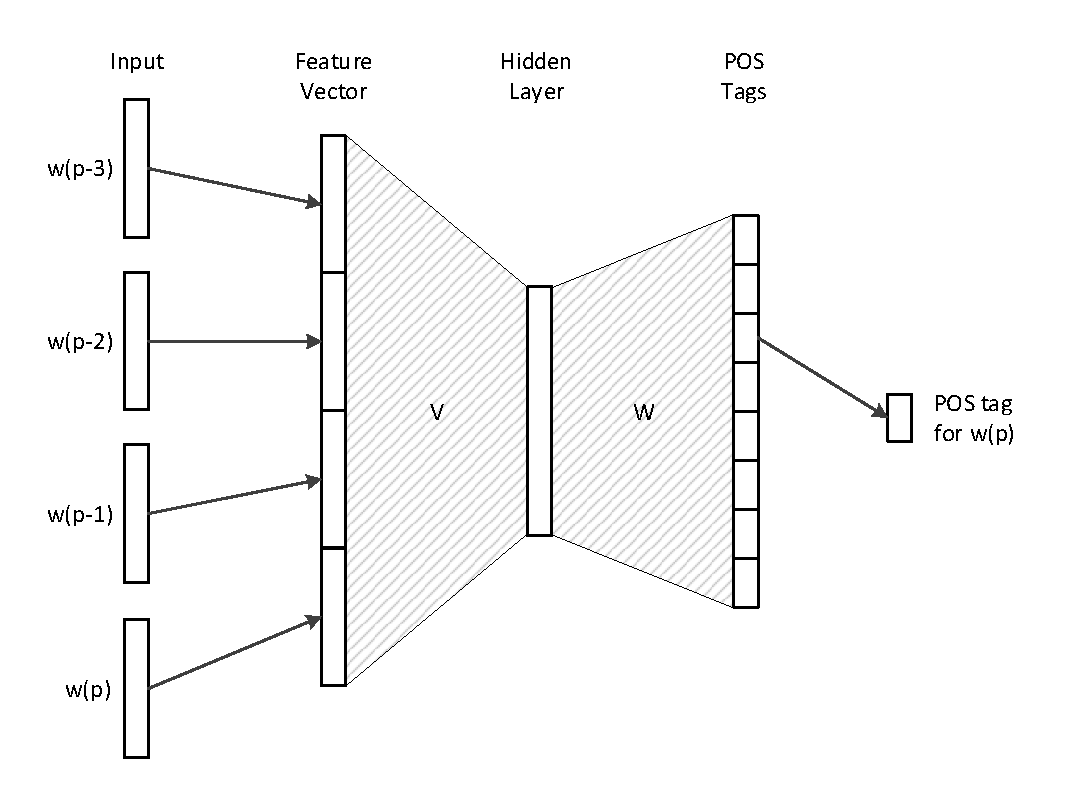
\includegraphics[width=\textwidth]{images/fnn_structure}
	\caption[Structure of a Feed-forward Neural Network]{The structure of a feed-forward neural network. The feature vector is built by the initial vectors of the corresponding input word on position \tt{p} and by its three predecessors (here as an example).}
	\label{f.fnn_structure}
\end{figure}

\subsection{Implementation}\label{c.postagging.fnn.implementation}
...

\section{Recurrent Neural Network Model}\label{c.postagging.rnn}
...

\subsection{Architecture}\label{c.postagging.rnn.architecture}
...
\begin{figure}[H]
	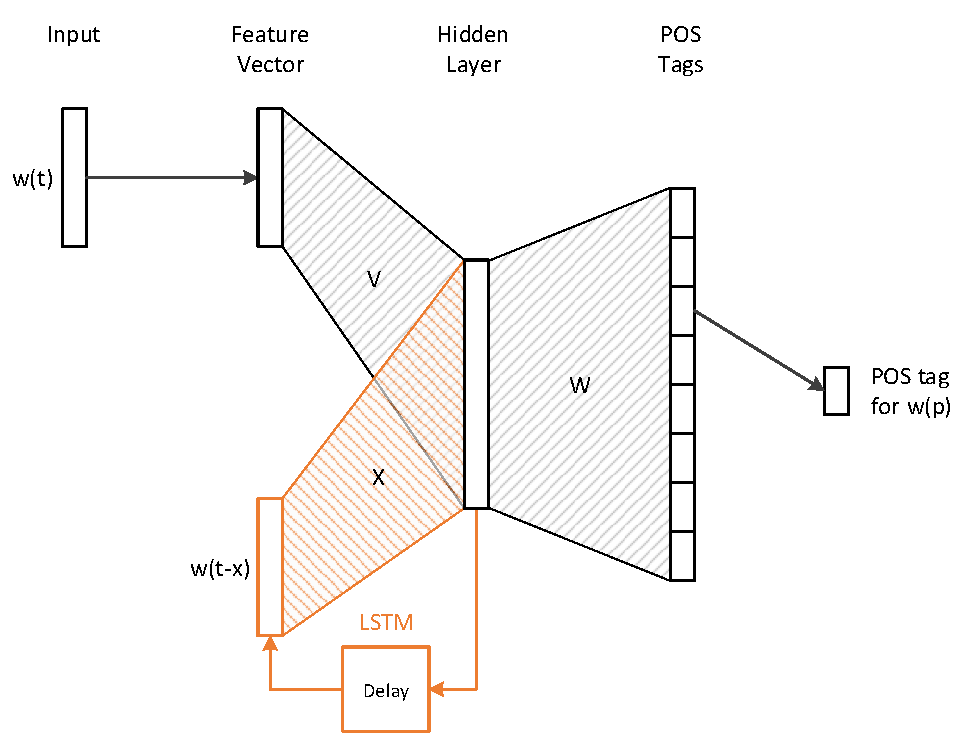
\includegraphics[width=\textwidth]{images/rnn_structure}
	\caption[Structure of a Recurrent Neural Network]{The structure of a recurrent neural network. The feature vector is the initial vector of the corresponding input word at time \tt{t}. The output of the hidden layer from previously trained words (here as an example at time \tt{x}) is fed back into the same hidden layer for the current word.}
	\label{f.rnn_structure}
\end{figure}

\subsection{Implementation}\label{c.postagging.rnn.implementation}
...

% ===================================================================================
\chapter{Training}\label{c.training}
...

\section{Data Retrieval}\label{c.training.data}
...

\section{Parameter Tuning}\label{c.training.tuning}
...

% ===================================================================================
\chapter{Evaluation and Comparison}\label{c.evaluation}
...

\section{Test Design}\label{c.evaluation.test}
...

% ===================================================================================
\chapter{Discussion and Conclusion}\label{c.conclusion}
...

\section{Summary}\label{c.conclusion.summary}
...

\section{Discussion}\label{c.conclusion.discussion}
...

\section{Future work}\label{c.conclusion.future}
...
\cite{michael2016}
\cite{mueller2015}
\cite{ma2000}
\cite{schmid1994}

% ===================================================================================
% \bibliographystyle{apalike}
% \bibliographystyle{plainnat}
% \bibliographystyle{abbrvnat}
% \bibliographystyle{unsrtnat}
% \bibliographystyle{alphadin}
\bibliographystyle{plain}
\bibliography{bibliography}

% ===================================================================================
\appendix
\chapter{First appendix}

\section{test}
...

\end{document}